%%%%%%%%%%%%%%%%%%%%%%% file template.tex %%%%%%%%%%%%%%%%%%%%%%%%%
%
% This is a general template file for the LaTeX package SVJour3
% for Springer journals.          Springer Heidelberg 2010/09/16
%
% Copy it to a new file with a new name and use it as the basis
% for your article. Delete % signs as needed.
%
% This template includes a few options for different layouts and
% content for various journals. Please consult a previous issue of
% your journal as needed.
%
%%%%%%%%%%%%%%%%%%%%%%%%%%%%%%%%%%%%%%%%%%%%%%%%%%%%%%%%%%%%%%%%%%%
%
% First comes an example EPS file -- just ignore it and
% proceed on the \documentclass line
% your LaTeX will extract the file if required
\begin{filecontents*}{example.eps}
%!PS-Adobe-3.0 EPSF-3.0
%%BoundingBox: 19 19 221 221
%%CreationDate: Mon Sep 29 1997
%%Creator: programmed by hand (JK)
%%EndComments
gsave
newpath
  20 20 moveto
  20 220 lineto
  220 220 lineto
  220 20 lineto
closepath
2 setlinewidth
gsave
  .4 setgray fill
grestore
stroke
grestore
\end{filecontents*}
%
\RequirePackage{fix-cm}
%
%\documentclass{svjour3}                     % onecolumn (standard format)
%\documentclass[smallcondensed]{svjour3}     % onecolumn (ditto)
\documentclass[smallextended, natbib]{svjour3}       % onecolumn (second format)
%\documentclass[twocolumn]{svjour3}          % twocolumn
%
\smartqed  % flush right qed marks, e.g. at end of proof
%
\usepackage{graphicx}
%\usepackage[numbers]{natbib} %TODO delete before submission
%TODO optimiere Zitierweise, fehlen Klammern um die Zitate?

%
 \usepackage{mathptmx}      % use Times fonts if available on your TeX system
%
% insert here the call for the packages your document requires
\usepackage{amsmath}

%\usepackage{latexsym}
% etc.
%
% please place your own definitions here and don't use \def but
% \newcommand{}{}
%
% Insert the name of "your journal" with
% \journalname{myjournal}
%
\begin{document}

\title{The Furuta Pendulum
%\thanks{Grants or other notes
%about the article that should go on the front page should be
%placed here. General acknowledgments should be placed at the end of the article.}
}
\subtitle{Technical Report}

%\titlerunning{Short form of title}        % if too long for running head

\author{Tabea Wilke \and Maximilian Gehrke \and Yannik Frisch}

%\authorrunning{Wilke, Gehrke, Frisch} % if too long for running head

\institute{F. Author \at
              first address \\
              Tel.: +123-45-678910\\
              Fax: +123-45-678910\\
              \email{fauthor@example.com}           %  \\
%             \emph{Present address:} of F. Author  %  if needed
           \and
           S. Author \at
              second address
}

\date{Received: date / Accepted: date}
% The correct dates will be entered by the editor


\maketitle

\begin{abstract}
The Furuta Pendulum is an example of a complex non-linear system and therefore 
of big interest in control system theory. It consists of one controllable arm 
rotating in the horizontal plane and one pendulum uncontrollably moving in the 
vertical plane, which is attached to the end of this arm.\\
The non-linearities result from an interplay between gravitational, coriolis, 
centrifugal forces and friction. \\
XX We present an overview over it's technical details and proposed algorithms to solve the control problem. XX
\keywords{First keyword \and Second keyword \and More}
% \PACS{PACS code1 \and PACS code2 \and more}
% \subclass{MSC code1 \and MSC code2 \and more}
\end{abstract}
\section{Introduction}
Many examples in the field of control engineering like aircraft landing, 
aircraft stabilizing and many more can be very well modelled by an inverted 
pendulum \citep{akhtaruzzaman2010modeling}. As a reaction to problems with the 
limited movement of the cart from 
the inverted pendulum, the furuta pendulum (also called rotary inverted 
pendulum) 
has been developed by 
\citeauthor{furuta1992swing}. The advantages of the furuta pendulum are that 
it 
needs less space and one moving arm is directly linked to the motor, therefore, 
the dynamics is less unmodeled thanks to a power transmission mechanism 
\citep{furuta1992swing}. \\
The furuta pendulum is an underactuated problem, this 
means that there  are two degrees of freedom ($\phi,\ \theta$), 
but only one arm is directly controlled by the motor. This is the one which 
changes the angle $\phi$ in the horizontal plane. The other arm called pendulum 
is attached to 
the end of the controlled arm and therefore is moved indirectly by it in the 
vertical plane with angle $\theta$ 
\citep{spong1998underactuated,tedrake2009underactuated}. The whole system is 
highly non-linear as a result of an interplay between gravitational, coriolis, 
friction and centrifugal forces \citep{izutsu2008swing}.
\begin{figure}[h]
	\centering
	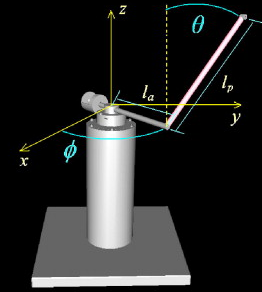
\includegraphics[width=0.5\linewidth]{pendulum}
	\caption{The furuta pendulum, figure from \cite{la2009new}}
	\label{fig:pendulum}
\end{figure}\\
Finally, there are two different types of control problems. First, bringing the 
flexible arm from a hanging position to a position which is nearly upright, 
further called "swing-up". Second, if the arm is nearly upright with low enough 
speed, balancing it to hold this state stable, called "stabilization". 
\subsection{Definitions}
The system consists of an arm with length $l_a$ mounted to a DC motor, which is 
able to apply a torque of $\tau$ to it. It has a mass of $m_a$ which is 
located at $l_1$ alongside the arm. Another arm with length $l_p$ and mass 
$m_p$ %located at $\frac{l_p}{2}$ 
is attached to the remaining side of the 
first arm. Both arms have a moment of inertia $J_a$ and $J_p$ respectively. The 
counter force to the input torque is the viscous damping $B_a$ because of the 
bearings of the motor. As the pendulum is not controlled directly, the only 
force it is applied to is damping at the connection to the arm $B_p$. The angle 
$\theta$ is zero if the pendulum is in an perfectly upright position.
The only influence we can take on the system is the voltage $V_m$ we give to 
the DC motor.
\section{Mathematical 
Modelling\protect\footnote[1]{\cite{akhtaruzzaman2010modeling,furuta1992swing,gafvert2016modelling,
		ozbek2010swing,zhang2011optimal,fairus2013fuzzy}}} 
For later derivation of the Lagrangian, the kinetic and potential engergies of 
the furuta pendulum are needed. Therefore, the kinematics of the pendulum's 
center of gravity can be described by 
\[\begin{cases}
x&=l_a\cos\phi-l_{p}\sin\theta\sin\phi \\ 
y&=l_a\sin\phi+l_{p}\sin\theta\cos\phi \\ 
z&=l_{p}\cos\theta
\end{cases} \] 
The relative velocity of the pendulum to the arm can be represented by 
\[ \begin{cases}
\dot{x}&=-l_a\ \sin \phi \dot{\phi}-l_{p}\ \cos\phi \sin\theta\dot{\phi}-l_{p} 
\ \sin\phi \cos\theta\dot{\theta} \\ 
\dot{y} &=l_a\ \cos\phi\dot{\phi}-l_{p} \ \sin\phi \sin\theta\dot{\phi}+l_{p} 
\ \cos\theta \cos\phi\dot{\theta} \\
 \dot{z}&=-l_{p} \ \sin\theta\dot{\theta}
\end{cases}\]
For the energy terms a squared velocity is needed, which is the scalar product 
of the squared velocities in all directions:
\begin{align*}v^2&=\dot{x}^2+\dot{y}^2+\dot{z}^2\\
&=(l_a^2+l_p^2\ 
\sin^2\theta)\dot{\phi}^2+l_p^2\dot{\theta}^2+2l_al_p\dot{\phi}\dot{\theta}\cos 
\theta\end{align*} %TODO ich kann die Herleitung dafür in den Anhang packen, 
%falls 
%gewünscht
First of all, we will derive the equations of motion through the Euler-Lagrange 
method. The Lagrangian function can be obtained by the difference of the 
kinetic and potential energies $L=T-V$, with $T$ as the total sum of the 
kinetic energies in the system and $V$ the total potential energies.\\
The only potential energy which is in the system is the one of the pendulum:
\[V_{total}=V_{pendulum}=m_pgz= m_pgl_{p}\cos\theta\]
Kinetic energy is available both in the arm and in the pendulum and is composed 
of the the sum of translation energy and rotational energy:
\begin{align*}
T_{arm}&=\frac{1}{2}J_a\dot{\phi}^2\\
T_{pendulum}&=\frac{1}{2}J_p\dot{\theta}^2+\frac{1}{2}m_pv^2\\
&= \frac{1}{2}J_p\dot{\theta}^2+\frac{1}{2}m_p\left((l_a^2+l_p^2\ 
\sin^2\theta)\dot{\phi}^2+l_p^2\dot{\theta}^2+2l_al_p\dot{\phi}\dot{\theta}\cos 
\theta\right)\\
T_{total}&= 
\frac{1}{2}J_a\dot{\phi}^2+\frac{1}{2}J_p\dot{\theta_0}^2+\frac{1}{2}m_p\left((l_a^2+l_p^2\
\sin^2\theta)\dot{\phi}^2+l_p^2\dot{\theta}^2+2l_al_p\dot{\phi}\dot{\theta}\cos 
\theta\right)
\end{align*}
From this the Lagrange Function arises:
\begin{align*}
L &=T_{total}-V_{total}\\
\begin{split}&=\frac{1}{2}J_a\dot{\phi}^2+\frac{1}{2}J_p\dot{\theta}^2+\frac{1}{2}m_p\left((l_a^2+l_p^2\
\sin^2\theta)\dot{\phi}^2+l_p^2\dot{\theta}^2+2l_al_p\dot{\phi}\dot{\theta}\cos 
\theta\right) \\&\quad - m_pgl_{p}\cos\theta\end{split}
\end{align*}
 Lagrange's 
Equation follows \[ 
\frac{d}{dt}\left(\frac{\partial L}{\partial 
	\dot{q_i}}\right)-\frac{\partial 
	L}{\partial 
	q_i}+\frac{\partial F}{\partial \dot{q_i}} =0\] Thereby, the variables 
	$q_i$ are called 
	generalized coordinates and $F$ is the friction in the system. 
	The friction in the system can be described by $B_p\dot{\theta}$ and $ 
	B_a\dot{\phi}$
	For 
the furuta pendulum the generalized coordinates are $\dot{q}(t)^T = 
\left[\frac{\partial 
	\phi(t)}{\partial t} \frac{\partial \theta(t)}{\partial t} \right]$ which 
	leads 
to 
\begin{align*}
\frac{\partial^2 L}{\partial t\partial \dot{\phi}}-\frac{\partial 
	L}{\partial \phi}&=\tau - B_a\dot{\phi}\\
\frac{\partial^2 L}{\partial t\partial \dot{\theta}}-\frac{\partial 
	L}{\partial \theta}&=-B_p\dot{\theta}
\end{align*}
The partial derivations of the Lagrangian for the generalized coordinates are:

\begin{align*}
	\frac{\partial L}{\partial \phi}&=0\\
	\frac{\partial L}{\partial 
	\dot{\phi}}&=\dot{\phi}(J_a+m_p(l_a^2+l_p^2\sin^2\theta))+\dot{\theta}(
	m_pl_al_p\cos\theta)\\
	\frac{\partial^2 L}{\partial t \partial \dot{\phi}}&= 
	\ddot{\phi}(J_a+m_p(l_a^2+l_p^2\sin^2 \theta))+l_p^2m_p\sin(2\theta)
	\dot{\phi}\dot{\theta}+m_pl_al_p(\cos 
	\theta\ddot{\theta}-sin\theta \dot{\theta}^2)\\
	\frac{\partial L}{\partial 
	\theta}&=\frac{1}{2}\dot{\phi}^2m_pl_p^2\sin(2\theta)-m_pl_al_psin\theta\dot{\phi}
	\dot{\theta}+m_pgl_psin\theta\\
	\frac{\partial L}{\partial 
		\dot{\theta}}&=\dot{\theta}(J_p+m_pl_p^2)+\dot{\phi}(m_pl_al_p\cos\theta)\\
	\frac{\partial^2 L}{\partial t \partial 
	\dot{\theta}}&=\ddot{\theta}(J_p+m_pl_p^2)+\ddot{\phi}m_pl_al_p\cos\theta-\dot{\phi}
	\dot{\theta}m_pl_al_p\sin\theta
\end{align*}
With this equations it is possible to derive the equations for the 
Euler-Lagrange's Equation:
\begin{align*}
\frac{\partial^2 L}{\partial t\partial\dot{\phi}}-\frac{\partial 
L}{\partial\dot{\phi}}&=\ddot{\phi}(J_a+m_p(l_a^2+l_p^2\sin^2 
\theta))+l_p^2m_p\sin(2\theta)
\dot{\phi}\dot{\theta}\\ &\quad + m_pl_al_p(\cos 
\theta\ddot{\theta}-sin\theta \dot{\theta}^2)\\
\frac{\partial^2 L}{\partial t\partial\dot{\theta}}-\frac{\partial 
L}{\partial\dot{\theta}}&=\ddot{\theta}(J_p+m_pl_p^2)+\ddot{\phi}m_pl_al_p\cos\theta-\frac{1}{2}\dot{\phi}^2m_pl_p^2\sin(2\theta)-m_pgl_psin\theta
\end{align*}
Putting this into a matrix form and filling in the friction, this results in 
the nonlinear equations of motion (EOM) for the furuta pendulum.
\begin{align*}
&\begin{bmatrix}
J_a+m_p(l_a^2+l_p^2\sin^2\theta)& \quad m_pl_al_p\cos\theta \\ 
m_pl_al_p\cos\theta& \quad J_p+m_pl_p^2 
\end{bmatrix} 
\begin{bmatrix}
\ddot{\phi}\\
\ddot{\theta}
\end{bmatrix} + \\
&\begin{bmatrix}
m_pl_p^2\sin(2\theta)\dot{\theta}- B_a& \quad -m_pl_al_p\sin \theta 
\dot{\theta}\\
-\frac{1}{2}m_pl_p^2\sin(2\theta)\dot{\phi} &\quad -B_p
\end{bmatrix}
\begin{bmatrix}
\dot{\phi}\\
\dot{\theta}
\end{bmatrix} +
\begin{bmatrix}
0\\
-m_pl_pg\sin\theta
\end{bmatrix}=\begin{bmatrix}
\tau \\
0
\end{bmatrix}
\end{align*}
\subsection{Linearization of the state-soace model}
As all equations of motion contain a part of a trigonometric function the 
equations are non-linear. There are several different methods to change the 
non-linear equations to linear ones. %TODO which ones
 For a linearization in the state-space the equation 
$\dot{x}=Ax+Bu+\tilde{d}$ is used. The linearization is done around the 
operating point \citep{rigatos2018nonlinear} which is the vertical inverted 
state and therefore, uses $\theta = 0$ and $\dot{\theta}=0$. This results in 
the following equations: %TODO Gleichung einfügen
The result is an linear form of the equations of motion which are very close to 
the system's description by the non-linear model, up to the first 25 degree 
which \citeauthor{kurode2011swing} showed.

\section{Pendulum Control}
The goal of controlling the furuta pendulum is to bring it from a hanging 
position into a vertical upright position. Therefore, it is necessary to 
generate enough energy to swing the pendulum up in a nearly upright position 
where the linear region begins \citep{kurode2011swing}. If this region is 
reached, the controller should change to the balancing mode to stabilize the 
upright position.\\
To check whether the controller needs to be switched from the swing-up task to 
the stabilize task, the switching criteria can for example be defined by:
\begin{align*}
\text{switching criteria}\footnotemark[2] =
\begin{cases} \text{stabilization} &\begin{cases}
|\theta|< \frac{\pi}{9} \ &\text{and}\  \dot{\theta} < 2.62\  \text{rad/sec}\\
|E-E_r|< 0.04 \ \text{Joule}\ &\text{and}\  \dot{\theta} < 2.62\  \text{rad/sec}
\end{cases}\\
\text{swing-up} & \text{otherwise}
\end{cases}
\end{align*}\footnotetext[2]{\cite{hamza2019current}}
\subsection{Swing-Up}
There are many different approaches for solving the swing-up task of the furuta 
pendulum, linear ones which use the linearized equations of motion, non-linear 
ones and model-free approaches. The classical way solving the swing-up task is 
an approach with energy control \citep{seman2013swinging}. Therefore, the sum 
of 
kinetic and potential energy of the pendulum is used to model which amount of 
energy should be added. The energy of the pendulum can be described by 
\[E = \frac{1}{2}J_p\theta^2+m_pgl_p(\cos \theta -1)\] which was already done 
by \citeauthor{aastrom2000swinging} for the normal pendulum.
The selection of the state without energy can be made differently, logically it 
is the upright state because there is no further need to add energy 
\citep{seman2013swinging}.\\
There are two different directions in which the 
energy can be supplied either the pendulum seems to be "pulled" or "pushed". To 
define this, the following term is used: $\text{sign}(\dot{\theta}\cos\theta)$ 
The velocity helps to find 
out whether the pendulum starts to swing in the opposite direction, the $\cos 
\theta$ defines if the pendulum is in the left or in the right half 
\citep{awtar2002inverted}. The magnitude of energy which should be provided is 
selected by an aggressivity factor and the difference of actual and desired 
system energy $k_a(E-E_0)$. The aggressivity factor handles the amount of input 
and thereby the number of oscillations which are needed to achieve the 
swing-up. Often there is also a saturation function which 
limits the signal to the maximum acceleration of the pendulum. The whole 
swing-up controller is then implemented by 
\begin{align*}
u = sat(k_a(E-E_0))\text{sign}(\dot{\theta}\cos\theta)
\end{align*}
\subsection{Stabilization}
There are many different approaches for solving the stabilization problem as 
well. The most common one is the linear quadratic regulation (LQR) because it 
guarantees the optimal solution \citep{hamza2019current}. But also the 
proportional integral derivative (PID) is often used because of its simplicity 
and robustness and also because of the usage in the industry 
\citep{hassanzadeh2011controller}. Nevertheless, there are a lot of other 
algorithms from sliding modes \citep{izutsu2008swing} to particle swarm 
optimization and other evolutionary algorithms 
\citep{hassanzadeh2011controller}.
%TODO LQR beschreiben

\section{Reinforcement Learning on the Furuta Pendulum}
In reinforcement learning the furuta pendulum has only a very small influence 
on the simulation and experimental research because of the complexity of the 
problem. Only a few algorithms were tested on it with divers results. Even if 
the robustness of the stabilization control should improve 
\citep{wang2004minimum}.\\
\citeauthor{hennig2011optimal} compares Gaussian process optimal learner with 
Kalman filter, TD($\lambda$) and as baseline full information. He used the same 
baseline function for all algorithms and collated the cumulated loss. 
Surprisingly, none of the methods could stabilize the swung up pendulum 
totally, even not the best method, the Gaussian process optimal learner.\\
Also an artificial neural network (ANN) was used to model the pendulum 
\citep{quyen2012rotary}. They worked with the voltage of the motor as input 
values and the angles of arm and pendulum as the output. Different numbers of 
hidden neurons were tested with the result that more neurons in the hidden 
layer led to a smaller mean squared error. The ANN could foresee the angle of 
the pendulum very well.\\
A good approach was done with recurrent neural networks and a Genetic Algorithm 
\citep{shojaei2011hybrid}. They used a recurrent neural network identifier and 
controller with a proportional integral derivative controller which was 
responsible for the feedback and the prediction in the derivative action.


\section{Conclusion}
The furuta pendulum is a very complex control problem which could be solved by 
a very wide variety of approaches. The control problem splits into two mayor 
problems the swing-up and the balancing task.

\bibliographystyle{spbasic}      % basic style, author-year citations
\bibliography{furuta.bib}   % name your BibTeX data base




\end{document}
% end of file template.tex

